\documentclass[12pt, onside]{book}
\usepackage{graphicx}
\usepackage[a4paper,width=150mm,top=25mm,bottom=25mm,bindingoffset=6mm]{geometry}
\usepackage[backend=biber, style=apa, autocite=inline]{biblatex}
\usepackage{hyperref}
\usepackage{xcolor}
\usepackage{sectsty}
\usepackage{listings}
\usepackage{amsmath}
\usepackage{array}
\usepackage{subcaption}
\usepackage[ruled,vlined, linesnumbered, algochapter]{algorithm2e}
\SetKwInput{KwInput}{Input}
\SetKwInput{KwOutput}{Output}
\definecolor{code}{gray}{0.95}
\definecolor{theme}{rgb}{0.09,0.43,0.37}
\definecolor{airforceblue}{rgb}{0.36, 0.54, 0.66}
\lstdefinestyle{pseudocode}{
	numbers=left,
	backgroundcolor=\color{code},
	tabsize = 2,
	numberstyle=\color{gray}
}
\allsectionsfont{\color{theme}}
\hypersetup{
    colorlinks=true,
    citecolor=theme,
    filecolor=black,
    linkcolor=theme,
    urlcolor= airforceblue,
}
\DeclareLanguageMapping{english}{english-apa}
\addbibresource{bibliography.bib}
\graphicspath{ {images/} }
\counterwithin{figure}{section}

\lstset{style=pseudocode}
\newcommand\themebold[1]{\textcolor{theme}{\textbf{#1}}}

\title{Clustering algorithms in the touristic sector}
\author{Argyro Sioziou}
\date{20 February 2020}

\begin{document}

\begin{titlepage}
    \begin{center}
        \vspace*{1cm}
 
        \Huge
        \themebold{Clustering algorithms in the touristic sector:}
 
        \vspace{0.5cm}
        \LARGE
        Case study on travel agency data
 
        \vspace{1.5cm}
 
        \themebold{Argyro Sioziou}

	\vspace{2.5cm}
 
        A thesis presented for the degree of\\
        Management Science and Technology
 
        \vspace{0.8cm}

	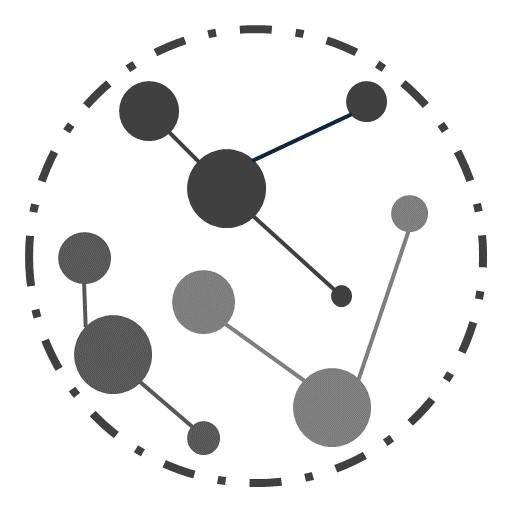
\includegraphics[width=0.4\textwidth]{clustering}

	\vfill

        \Large
        Management Science and Technology\\
        Athens University of Economics and Business\\
        Greece\\
        20/02/2020

	\vspace{2.5cm}
 
    \end{center}
\end{titlepage}

\begin{center}
    \Large
    \themebold{Clustering algorithms in the touristic sector}
    
    \vspace{0.4cm}
    \large
    Case study on travel agency data
    
    \vspace{0.4cm}
    \themebold{Argyro Sioziou}
    
    \vspace{1.5cm}
    \themebold{Abstract} 
\\
\vspace{25mm}
Machine learning, and especially clustering, are nowadays broadly used by businesses of many different sectors, to extract knowledge from their data, and use it in favor of themselves and their customers. The tourism sector also seeks to exploit its data and gain insights from them. Though, this sector, deals with the problem that its data in its majority are categorical, and therefore harder to analyze. In this thesis, an introduction of machine learning and clustering is made and two algorithms are thoroughly analyzed. Afterward, a case study is presented that shows the importance of clustering techniques for tourism, using the data of a travel agency. The case study proves, that even though categorical data make it harder to extract meaningful results, machine learning still constitutes a very useful way to guide tourism businesses through their decisions. 
\end{center}

\tableofcontents

\chapter{INTRODUCTION}
\section{Research Motivation}
The fourth industrial revolution has come with many new technologies, and even though it has just begun, it is affecting people's lives and companies' behaviors in many aspects \autocite{revolution}. The latter are searching for new ways to address the former and engage them, while their expectations are continuously increasing. This leads companies of many industries, including tourism, to intend to deliver personalized experiences, using tools like marketing \autocite{engagement}. At the same time, the available data volume is increasing rapidly, giving the ability to enterprises worldwide to extract knowledge from them and create value \autocite{bigdata}.
This plethora of data provides an opportunity for marketers of the tourism sector, amongst others, to perform better segmentation, and get insights into their customers' needs using cluster analysis \autocite{fuzzyturism}. The results of such techniques can also help businesses of the industry in their decision-making process and the creation of competitive advantage \autocite{advantage}. However, this task is not that simple. Turistic data are to a large extent qualitative, which makes it hard for analysts to extract the maximum knowledge from them since clustering algorithms are in their majority used with quantitive data \autocite{categorical}. \\
The process of eventually managing to extract the wanted information seems challenging. We could suppose though, that with the proper handling the results could prove rewarding for both the businesses and the customers. Based on this conjecture, we try to respond to this thesis how could a company of the tourism industry, using cluster analysis, take deal with its complex data and create value for itself and its customers.
\section{Research Methology}
To respond to the research objectives and questions, which were defined in the previous section, data of the backoffice system of a travel agency were used as a case study. The data were cleaned, reformed and metadata were extracted from them. The majority of the data were categorical. Next, two clustering algorithms were used to create meaningful groups. Before the analysis, a research on the algorithms was done in order to better understand their functionality. Afterward their results were analyzed and compared in order to conclude whether the results could be valueble and how.
\section{Thesis Outline}
The main goal of this thesis is to experiment with the use of clustering algorithms with categorical data and identify the value of its results in the formation of services, and the creation of marketing strategies in the tourism sector. Firstly, it defines machine learning and its categories, concentrating mainly on clustering and its applications in various sectors. Next, it analyses more in-depth two clustering methods, the Kmeans, and Agglomerative clustering. Further, in the last section of the research background, a thorough description of two clustering applications in the tourism sector are illustrated. Then, the case study description, available data, methodology, and results are presented. In conclusion, the results of the two algorithms are compared and their avail is discussed.

\chapter{BACKGROUND}
\section{Overview}

\subsection{Machine Learning}
Machine learning is the field of study that focuses on training machines (e.g., computers) to identify patterns and derive logical conclusions \autocite{machDef}. It is technically an imitation of the human learning process and can be divided into different types based on the approach it uses to train the algorithm \autocite[5]{chapman}. The two main types are supervised and unsupervised learning \autocite[43]{dunham}: \\
\begin{itemize}
\item Supervised learning is used to classify instances to already known categories based on their characteristics. Algorithms that belong to this type are first trained on an already labeled with the possible categories dataset and, afterward, use their gained knowledge to classify new unlabeled datasets \autocite[24]{han}. Technically it is like a human trying to learn by first looking at all the correct answers and then, based on them, try to classify new ones \autocite[5]{chapman}. For example, a supervised learning problem would be images, each one containing one hand-written digit, and its label the number to which it corresponds. After training the algorithm with a labeled set, the algorithm would be capable of recognizing digits on images. \\
\item Unsupervised learning, on the other side, is used to group data without knowing the labels beforehand and without any training proceeding. This type of learning allows the model to learn by itself. Usually, a person with knowledge in the sector is needed to interpret and extract the knowledge from the created groups \autocite[25]{han}. In this case, a human would only know whether or not his answer is correct, but nothing about the way to the right answer \autocite[5]{chapman}. The above example using unsupervised learning would be giving as input the images to the algorithm without labeling the digits. The expected output would be ten clusters, each one corresponding to one of the digits from zero to nine. A person inspecting the results would be in the position to recognize which is the digit shown on the images of each cluster. \\
\end{itemize}
Apart from those two main categories, two additional categories are worth mentioning, semi-supervised learning, and reinforcement learning. \\
\begin{itemize}
\item Semi-supervised learning falls between the above two types. It consists of a small amount of labeled data and a large amount of unlabeled data. The labeled data serve as initial training, and the results are using the unlabeled data to improve the process and, on many occasions, spot outliers \autocite[25]{han}. Following \textcite{chapman}'s ratiocination, in real life, it would look like a person given a few correct answers as a starting point to solve more complex questions. Using the digits example, let us suppose that labeling all the pictures would be a very costly procedure, therefore someone would label a small amount of the images to use as the training set, and afterward apply the algorithm to the rest of the images to improve the model.
\item Reinforcement learning is a more interactive method, as opposed to the previous ones. It uses unlabeled data and requires rewards or penalties based on its behavior. This type of machine learning takes decisions that lead to the maximization of the reward taken (e.g., a numerical value) \autocite[2-3]{rein}. Similarly to unsupervised learning, it is like giving feedback to a person, but not by telling it whether the answer is correct or not, but by grading its performance. Then that person using its sought knowledge would try to improve itself \autocite[5]{chapman}. Therefore, the digits paradigm would be similar to the one of unsupervised learning. However, instead of trying to discover hidden patterns, it would try to find the output with the maximized reward (or minimized penalty), making different decisions based on its previous experience.
\end{itemize}

\begin{figure}[ht]
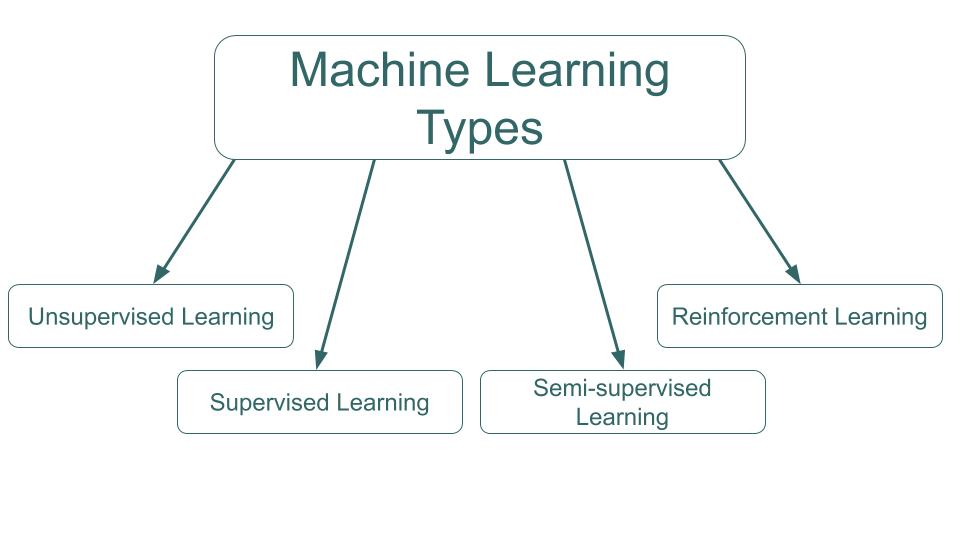
\includegraphics[width=\textwidth]{mach_learn_types}
\caption{Types of machine learning.}
\label{fig:types}
\end{figure}

\subsection{Clustering}
As indicated by the definitions given by \textcite{dunham} and \textcite{tanSteinKum}, clustering or cluster analysis is a type of unsupervised machine learning. It groups instances to create coherent sets based on their similarities and dissimilarities. The aim is that instances that belong to the same sets are as much alike and as much different from the instances of the other sets as possible \autocite{dunham, tanSteinKum}. \\
As \textcite{kantar} claims, humans are capable of detecting natural clusters from given data and compete with the clusters created by algorithms up until three-dimensional data. In real life, though, the dimensionality of the data examined is usually much higher than that, and therefore, if the cluster analysis were possible to be done by a human, it would not be as efficient \autocite[250]{kantar}. Since it is not humans that perform clustering, but algorithms, unexpected groups, and patterns can be discovered \autocite[444]{han}. \\
The usefulness of cluster analysis can be confirmed from its numerous applications in various fields of study. Some of them are mentioned by \textcite{clAnalysis}. Some of them briefly described are the following:
\begin{itemize}
\item Market research. A market researcher may want to use clustering to segment its audience and form its target groups. Furthermore, it can be useful to find the correlations between the financial measures of a company to its stock performance. \textcite{chakrapani} describes an example in the market of sports cars. Whether a person will buy a sports car is not affected by demographics, but by its lifestyle, clustering can help to spot those lifestyles that lead to such a purchase \autocite[9]{clAnalysis}.
\item Astronomy. Astronomers need to discover distinct groups out of large data sets. For example, on \textcite{astronomy}'s application, stars could be divided into groups differentiated by their volume and size based on their velocities \autocite[10]{clAnalysis}.
\item Psychiatry. Cluster analysis can group mental illnesses, detect patterns in people that commit suicide, investigate parasuicidal patients, and classify eating disorders. By further research on the results, new approaches can be proposed. \textcite{psychiatry} found three different types of people that attempt suicide. They differ mainly on the cruelty of the methods they chose and their motivation behind the attempt \autocite[10]{clAnalysis}.
\item Bioinformatics and genetics. As \textcite{clAnalysis} explain, the genetic code is complex, and its variations are responsible for the differences between organisms. In each cell, different genes are expressed, resulting in the production of several proteins. Combining different cell types makes an organism functional. In the case of alterations in the genetic code or malfunctions in those processes, diseases occur. Through clustering, it is possible to study the cause of a disease, investigate inheritance, discover the functionality of new gene sequences, and make research more efficient and affordable \autocite[12-13]{clAnalysis}. \textcite{bioinformatics} used clustering in their article to group genes that follow similar expression patterns in order to decrypt a gene's functionalities and regulative mechanisms \autocite{bioinformatics}.
\end{itemize}
Additional applications of clustering in the touristic sector will be analyzed more in-depth in section \ref{applications}.

\subsection{Types of Clustering}
Clustering algorithms can be categorized based on two criterions. The first one is the relationships between the produced clusters of one iteration with the ones of a previous iteration. The second one is the number of clusters an instance can be a part of. \\
Based on the first criterion, \textcite{tanSteinKum} describe the following types: \\
\begin{itemize}
\item Partitional clustering is a type of clustering which allows no overlapping between two or more sets of clusters, hence partitions the initial set to independent sets. This means that each instance can be part of exactly one cluster \autocite[492]{tanSteinKum}. \\
\item Hierarchical clustering produces clusters in each iteration, which are subsets of a cluster of the previous iteration. This can occur by starting from one cluster, which contains all instances, and repeatedly partition the available clusters to even smaller ones \autocite[492]{tanSteinKum}. \\
\end{itemize}
\textcite{tanSteinKum} mention three more types of clustering in their book, which are formed based on the second criterion and are the following: \\
\begin{itemize}
\item Exclusive clustering signifies that an instance can only be a part of only one cluster \autocite[492]{tanSteinKum}. Let us define the binary variables \(x_{i}\) for each instance \(x \in X \), where \(X\) are all the instances. If an instance \(x\) belongs to the \(i^{th}\) cluster \(x_{i}\) is set equal to 1, otherwise to 0. Then, if the number of clusters is \(n\), we can describe each cluster by the function:
\begin{eqnarray*}
C_{i} = \{(x, x_{i})|x \in X\}
\end{eqnarray*}
where \(C_{i}\) is the \(i^{th}\) cluster, and which has the following restrictions:
\begin{eqnarray*}
\sum_{i=0}^{n} x_{i} = 1, x_{i} \in \{0,1\}
\end{eqnarray*}
\item Overlapping or non-exclusive clustering signifies that an instance can be part of more than one cluster \autocite[492]{tanSteinKum}. We can describe each cluster the same way we did in exclusive clustering, just by adjusting the restrictions:
\begin{eqnarray*}
C_{i} = \{(x, x_{i})|x \in X\} \\
\sum_{i=0}^{n} x_{i} \geq 1, x_{i} \in \{0,1\}
\end{eqnarray*}
where \(C_{i}\) is the \(i^{th}\) cluster, \(x\) is a specific instance, \(x_{i}\) is the binary variable that describes \(x\) in the \(i^{th}\) cluster, \(X\) are all the instances and \(n\) is the number of clusters.
\item Fuzzy clustering signifies that every instance belongs to all the clusters \autocite[492]{tanSteinKum}. As \textcite{kantar} explains, the function that shows the membership of an element inside a cluster is called membership function (MF). The value of the MF that describes a given instance is a number between [0,1]. Each cluster can be described as follows:
\begin{eqnarray*}
C_{i} = \{(x, \mu_{C}[x])|x \in X\}
\end{eqnarray*}
where \(C_{i}\) is the \(i^{th}\) cluster, \(x\) is a specific instance, \(\mu\) is the MF function, and \( X\) is the set that contains all the instances \autocite[416]{kantar}.
\end{itemize}

\section{K-means}
K-means is a prototype-based, iterative algorithm in which instances are assigned to a cluster in each iteration. The basic algorithm requires as input K points, called centroids, where K is the number of the desired clusters. To define the cluster to which one instance belongs to, the algorithm calculates its distance from all the centroids and assigns it to the closest one. Finally, using the produced clusters calculates the new centroids and repeats until it reaches the desired set. Each cluster's mean needs to be defined and recalculated in each iteration to redefine the new centroids \autocite{dunham, tanSteinKum}. \\
\textcite{euclidean} explain that K-means is practically a minimization problem. The objective function (the function to be minimized) is the function that calculates the distances between one instance and its cluster's centroid. The smallest the sum of the distances of one cluster's centroid to its instances, the highest the homogeneity of the cluster \autocite[2]{euclidean}. \\
Disimalirites between data objects are their distance \autocite[69]{tanSteinKum}, though there are many different methods of calculating the distance between two instances, the most common one used is the Euclidean distance \autocite[648]{survey}. Using the Euclidean distance to calculate the distances between the centroid of a cluster, and the rest of the cluster's instances, for a one-dimensional dataset, the model is as follows:
\begin{eqnarray*}
d_{ij} = \sqrt{(c_{i}-x_{j})^2}
\end{eqnarray*}
where \(d_{ij}\) is the distance of the \(j^{th}\) element from the \(i^{th}\) cluster, \(c_{i}\) is the \(i^{th}\) centroid, and \(x_{j}\) is the \(j^{th}\) element \autocite[69]{tanSteinKum}. \\
In the simple case where there is only one numerical value describing each instance the cluster mean can use the basic mean definition from statistics as follows: \\
\begin{eqnarray*}
m_{i} = \frac{1}{m}\sum_{j=1}^{m}(x_{ij})
\end{eqnarray*}
where \(m_{i}\) is the mean of the \(i^{th}\) cluster, \(m\) is the number of instances that belong to the \(i^{th}\) cluster, and \(x_{ij}\) is the \(j^{th}\) instance of the \(i^{th}\) cluster \autocite[140]{dunham}. \\
As \textcite{dunham} describes, the termination techniques of the algorithm may vary. It could be that the clusters of each iteration are the same or almost the same or that the algorithm terminates after a fixed number of iterations \autocite[140]{dunham}.  
\begin{algorithm}
\SetAlgoLined
\KwInput{\(D=\{x_{1},x_{2},...,x_{n}\} \)\newline
K initial centroids
}
\KwOutput{K cluster sets}
\While{termination condition is not reached}
{
Assign each element to the cluster of the closest centroid.\\
Recompute the new centroids.
}
\caption{K-means}\label{alg:kmeans}
\end{algorithm} \\
Algorithm \ref{alg:kmeans} shows the K-means' basic steps \autocite{dunham, tanSteinKum}. \\
The algorithm's time complexity is O(tkn), where t is the number of iterations, n the number of elements, and k the number of clusters. \autocite[141]{dunham}. It is considered to produce good results and handles better storage and noise compared to some hierarchical agglomerative algorithms \autocite[526]{tanSteinKum}. On the other side, it is not very scalable and time-efficient \autocite[141]{dunham}. Furthermore, outliers need to be handled exclusively in order for the clusters to be representative \autocite[506]{tanSteinKum}.Finally, since K-means bases on the euclidean measure, it works well with globular data, but not that well with other geometrical shapes nor with multi-dimensional(categorical) data \autocite[647, 649]{survey}. 
\section{Applications in the touristic sector}
\label{applications}
\subsection{Benefit Segmentation}
As \textcite{data-drivenSegmentation} states, companies all around the globe use market segmentation to target their audiences more effectively and consume their resources more efficiently. Cluster analysis is a useful tool for the creation of those segments to create groups of people that seek similar benefits from their travel experiences. These groups not only help in the formation of marketing strategies but also to products that offer higher fulfillment to their consumers \autocite[17]{data-drivenSegmentation}. This type of segmentation was introduced by \textcite{Haley} in 1968 and is called benefit segmentation. The need for the creation of a new way of grouping target groups arose from the fact that tourists' behavior is mainly determined by the benefits they seek to satisfy and not by descriptive factors \autocite[31]{Haley}. \\
A sample application of benefit segmentation using cluster analysis describe \textcite{finland} in their article. Data about tourists were gathered in the region of Savonlinna, Finland, during the period with the highest footfall of the year through electronic questionnaires. The research aims to find the different segments of tourists based on the benefits they seek and then examine the interest of each segment on wellness holidays. \\
For the segment formulation, they used two algorithms, one hierarchical to find the best number of clusters, and K-means to create the clusters. The solution they proposed contained four distinct clusters. From the four clusters, two of them seemed to have a higher preference for wellness services, as designated by \textcite{finland} 'Culturals' and 'Sightseers'. Both clusters portrayed people that seem to favor attractions and also have a tendency to go back to the same destination for their vacation. Additionally, the 'Culturals' show a preference for cultural activities, where 'Sightseers' show a preference for sightseeing activities. The illustrated interpretation of the results is that the previous approach, which promoted wellbeing products based on nature, might not be the most appropriate. The suggested alternative claims that combining wellbeing with history, culture, diverse experiences, and attractions could be more efficient \autocite[308-312]{finland}. \\
Another sample application that focuses more on the nature of the data to be analyzed describes \textcite{categorical}. Commonly, collected touristic data come from surveys, which, to a great extent, contain qualitative data. Furthermore, for the market segmentation to produce more representative results, many attributes should be used. Even so, most clustering methods used by marketers do not work well nor with multidimensional nor with categorical data \autocite[391]{categorical}. \\
\textcite{categorical} used a Bed and Breakfast (B\&B) survey in order to illustrate a more reliable way to deal with this type of data. First, they used multiple correspondence analysis (MCA) to produce some initial cluster groups, get a visualization of them, and understand them. Afterward, they performed cluster analysis, using the k-means algorithm, in order to find the market segments. They concluded in four clusters, from which the three of them seemed to be worthy of further analysis. The other cluster did not contain enough data to lead to meaningful interpretation. The first of the three segments contained respondents who were seeking a romantic experience and were less likely to return to the B\&B. Also, they were not very concerned about the cost and amenities provided. Tourists of the second cluster were looking for cozier, more peaceful, nature-related options and were more likely to go back to the same place if they liked it. They also preferred to take part in energetic activities and, similarly to the first cluster, do not care so much about price and amenities. The third cluster was technically a mixture of the two previous ones. The distinguishing factor was the eagerness of the people of the latter to socialize and the importance of price, value factors \autocite[394-395]{categorical}. \\
Taking into consideration the results of the k-means \textcite{categorical} used the geographical characteristics of each cluster and suggested the usage of different marketing approaches on each of the three regions that the respondents came from (Wisconsin, Minnesota, Illinois). The B\&B owners made some changes based on the formed clusters to improve their customer satisfaction. For example, they decided to offer a private breakfast to the first cluster, add more activities to please the second cluster, and provide information about social events to the people of the last cluster. Furthermore, they were planning on changing their marketing strategy based on the demographics provided by the research to better target their audience \autocite[395-396]{categorical}.

\chapter{CASE STUDY: CLUSTER ANALYSIS ON TRAVEL AGENCY'S DATA}
\section{Data}

\subsection{Description}
The data used for clustering were drawn from the back office system of a travel agency in Parga, Greece. The majority of the data are about hotel reservations. The rest are about excursions and transfers. The back office uses a relational database to store its data. After thoroughly examining the available tables, only a few of them were kept for the analysis, the ones that seemed to have the most analytical value. Their relationships are shown in the following simplified diagram. \\
\begin{figure}[ht]
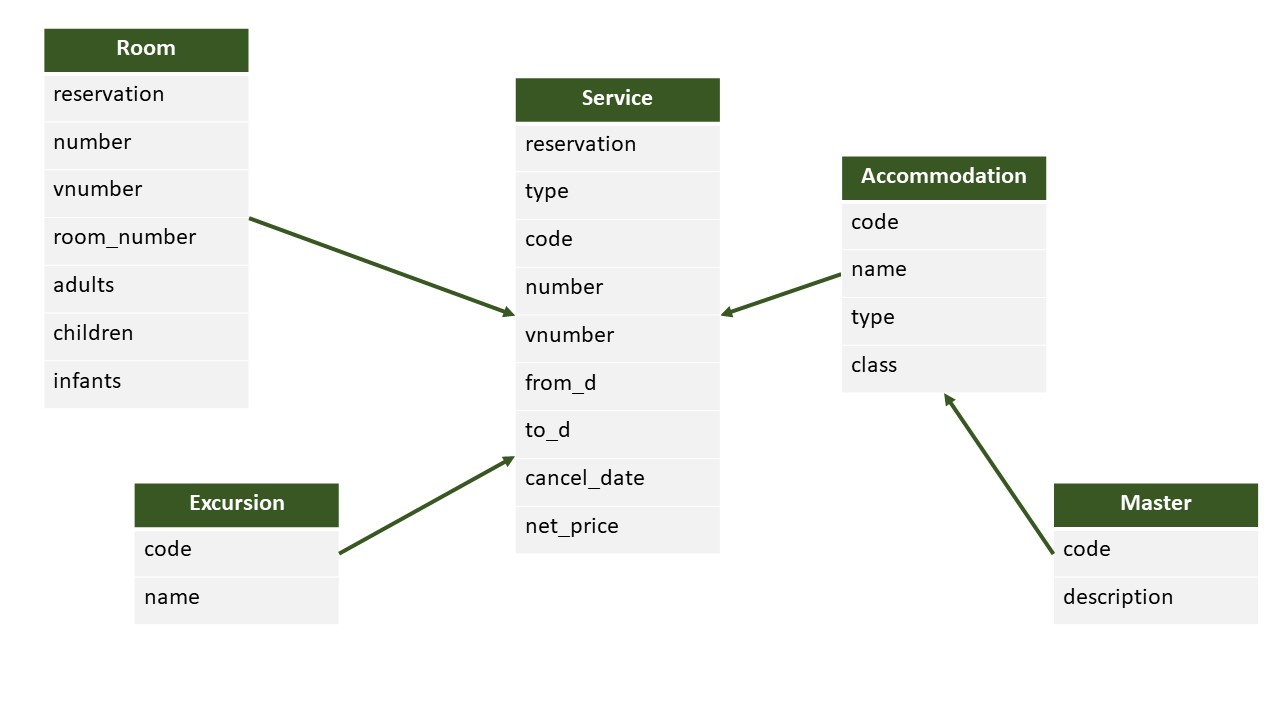
\includegraphics[width=\textwidth]{erp}
\caption{Relationships diagram.}
\label{fig:erp}
\end{figure}
\\
One reservation may consist of many services (e.g., hotel reservation, excursion activity). For each service booked, there is at least one corresponding row on the 'Service' table that contains its details in a total of sixty-seven columns. Eleven of them were used and are explained in table \ref{tab:service}. \\
\begin{table}[h!]
\begin{center}
\begin{tabular}{l | p{12cm}}
\textcolor{theme}{\textbf{Column}} & \textcolor{theme}{\textbf{Description}}\\
\hline
reservation & Service's reservation identifier.\\
\hline
type & Service type. Can be either hotel(HTL), excursion(EXC) or transfer(TRF).\\
\hline
code & Service code from either 'Excursion', 'Hotel', or 'Transfer' tables.\\
\hline
number & Service number. The service's identifier number per reservation.\\
\hline
vnumber & Service vnumber. A number starting from one for each service per reservation. Whenever the service is edited a new row is created with the updated details and vnumber incremented by one.\\
\hline
fromd & Service's starting date.\\
\hline
tod & Service's ending date.\\
\hline
net\_price & The total price of the booked service.\\
\hline
status & Reservation status. Can be either canceled(CL) or confirmed(CF). \\
\hline
customer\_id & Customer's identifier.\\
\hline
\end{tabular}
\caption{Service table.}
\label{tab:service}
\end{center}
\end{table}
\\
Whenever an accommodation service is booked, the "Accommodation"(\ref{tab:accommodation}) table, holds the information that describes it. Using the service code set on the "Service" table the corresponding accommodation can be found. \\
\begin{table}[h!]
\begin{center}
\begin{tabular}{l | p{12cm}}
\textcolor{theme}{\textbf{Column}} & \textcolor{theme}{\textbf{Description}}\\
\hline
code & Accommodation identifier.\\
\hline
name & Accommodation name.\\
\hline
type & Accommodation type identifier. Categorical value that shows the type of the accommodation. \\
\hline
class & Accommodation class identifier. Categorical value that shows the quality of the accommodation. \\
\hline
\end{tabular}
\caption{Accommodation table.}
\label{tab:accommodation}
\end{center}
\end{table}
\\
The "Master"(\ref{tab:master}) table contains several codes, and its descriptions, that can be found on many tables of the database, including the accommodation class and type codes. \\
\begin{table}[h!]
\begin{center}
\begin{tabular}{l | p{12cm}}
\textcolor{theme}{\textbf{Column}} & \textcolor{theme}{\textbf{Description}}\\
\hline
code & A code.\\
\hline
description & Code's description.\\
\hline
\end{tabular}
\caption{Master table.}
\label{tab:master}
\end{center}
\end{table}
\\
Furthermore, whenever an accommodation is booked, at least one new row is entered in 'Room' table. These rows contain the information of the booked rooms of the accommodation, as described in table \ref{tab:room}. \\
\begin{table}[h!]
\begin{center}
\begin{tabular}{l | p{12cm}}
\textcolor{theme}{\textbf{Column}} & \textcolor{theme}{\textbf{Description}}\\
\hline
reservation & Service's reservation identifier.\\
\hline
number & Service number. The service's identifier number per reservation.\\
\hline
vnumber & Service vnumber. A number starting from one for each service per reservation. Whenever the service is edited a new row is created with the updated details and vnumber incremented by one.\\
\hline
room\_number & The number of rooms contained in this service booking with this specific composition.\\
\hline
adults & The number of adults in this room.\\
\hline
children & The number of children in this room.\\
\hline
infants & The number of infants in this room.\\
\hline
\end{tabular}
\caption{Room table.}
\label{tab:room}
\end{center}
\end{table}
\\
Similarly to an accommodation booking, when an excurision is booked its details can be found through the service code of "Service" table in table \ref{tab:excursion}. \\
\begin{table}[h!]
\begin{center}
\begin{tabular}{l | p{12cm}}
\textcolor{theme}{\textbf{Column}} & \textcolor{theme}{\textbf{Description}}\\
\hline
code & Excursion identifier.\\
\hline
name & Excursion name.\\
\hline
\end{tabular}
\caption{Excursion table.}
\label{tab:excursion}
\end{center}
\end{table}
\\
\subsection{Processing and reforming}
After cleaning the data and before performing the analysis, some additional preprocessing was done. This preprocessing contained the creation of new columns and tranformation of categorical data to numerical, ordinal whenever that was possible.Eventually, the tables were reformed to a flat structure. The additional data were used both for the analysis and the interpretation of the results. \\
First of all, the service booking dates were used in order to define the season status of the trip. The season status can either be low, medium or high, and is used to show whether, in a certain period, a small or a big number of reservations is expected. As defined from the travel agency, high season is during Christmas and Easter(in this case orthodox) holidays and from the 10th of July to the end of August. Medium season are considered September, June and from the 1st until the 9th of July. The rest of the year is considered low season. Furthermore, in order to keep each booked service only once, on its final state, only the maximum vnumber was kept for each service. Finally, for the accommodation services, to get a more representative value of the service,  the price per person per night was calculated. \\
As shown in figure \Nameref{fig:erp}, the 'Room' table contains information with regard to its composition. Instead of just using the number of adults and children a composition tag was created. The terms used by the travel agency to describe the composition are family, couple, single, crew and group. For interpration purposes these tags were added to the room data. \\
As already mentioned, information about the type and class can be drawn from the 'Master' table. The descriptions of the codes by themeselves provide many verbal information that can be summarized to create universal tags for the accommodations. Therefore, using those descriptions, five type tags were created, hotel, studio, apartment, house and villa, and three class tags, A(high class), B(medium class) or C(low class). The class tags were represented by numerical values for the analysis.

\section{Kmeans}
\section{Agglomerative Clustering}


\chapter{CONCLUSIONS}
\section{Comparing Results}
The task of dealing with categorical data is demanding and requires good data manipulation to produce satisfactory results. Through the usage of the two algorithms, we could say that both of them worked pretty well with them and provided useful information. Especially Kmeans, even though it is not considered to work well with this type of data, produced the best results out of two, managing to recognize all the four groups. \\
Indeed the results could have been better if the categorical data did not affect them that much. Still, the travel agency can take advantage of the outcome to adjust both its product and marketing strategy in favor of the clusters 'Luxury trip' and 'Relaxing vacation' to become more competitive in the touristic market and increase its revenue.
\section{Restrictions}
Even though the dataset contained a sufficient volume of data, these were not evenly distributed throughout the different kinds of information. The data about the accommodations were severely outnumbering the excursion data. This resulted in the latter not playing any role in the cluster formation. The main reason why the excursion data were insufficient was due to the misuse of the backoffice system. Initially, a large amount of excursion data were available, but not properly inserted, at the time of the reservation, in the system and therefore was not possible to connect them to their corresponding accommodation reservation. \\
Furthermore, as mentioned, the clusters were to a large extent formed by the type of accommodation. If the type of accommodation was to be translated as the benefits that a client seeks on, for example, renting a studio instead of an apartment the results could offer a better picture of the factors that affect a traveler's decisions. This type of information was not currently available.
\section{Future Work}
The analysis did result in useful insights for the agency. Additional analysis though could be done if the current dataset was enriched by survey data given to the travelers. These data could be about the benefits sought from their trips, and the factors that lead them to choose the services they chose. In this way, some categorical data could be converted to ordinal and the analysis would produce better results. \\
Furthermore, the same way this analysis was mainly focused on the accommodations since they could not be combined with all the equivalent excursions, a second analysis could be conducted based on the excursions. This analysis could produce excursions bundles to be promoted together. Finally, the agency's portfolio of excursions could be expanded based on the most profitable ones.

\printbibliography
\addcontentsline{toc}{section}{Bibliography}
\end{document}